\chapter{Pregled modela}
\label{ch:pregled-modela}

Poglejmo si še eno zanimivo kombinacijo gradnikov: Tree Viewer in Scatter Plot. V Scatter Plotu najdite najboljšo vizualizacijo podatkov, torej tako, ki najlepše loči med razredi. Nato povežite Tree Viewer v Scatter Plot. Ob izboru katerekoli veje iz drevesa, se bodo v Scatter Plot obarvale točke, ki pripadajo izbrani veji.\marginnote{Kadar je mogoče, vizualizacije v Orangeu podpirajo izbor in pošiljanje podmnožic. Iskanje zanimivih podmnožic in analiziranje njihovih lastnosti je ključen del raziskovalne analize podatkov, pristopa, ki ga priporoča guru vizualizacije podatkov Edward Tufte.}

\begin{figure}[h]
    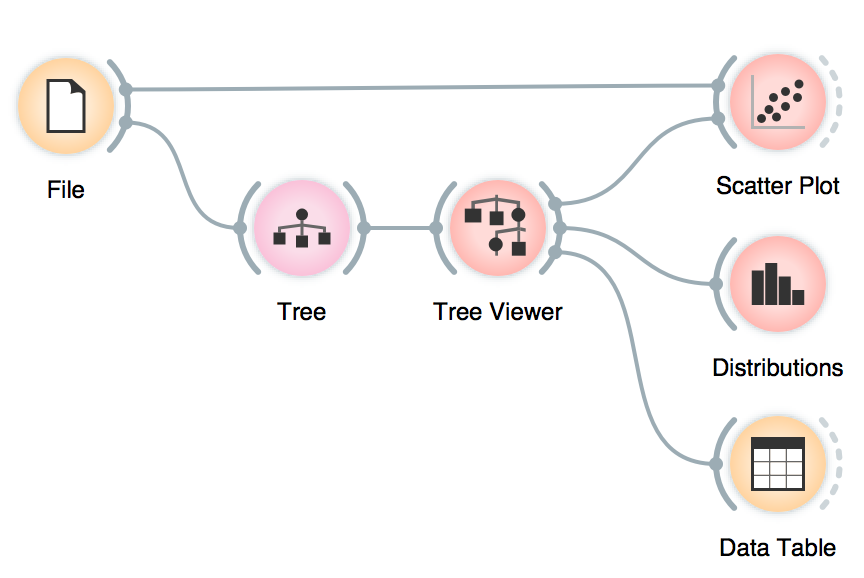
\includegraphics[width=0.8\linewidth]{workflow.png}
    \caption{$\;$}
\end{figure}

Za zabavo smo vključili še nekaj gradnikov v delotok. Tree Viewer izbere podmnožico, ki ustreza pravilom, kot jih poda model.

\begin{figure}[h]
    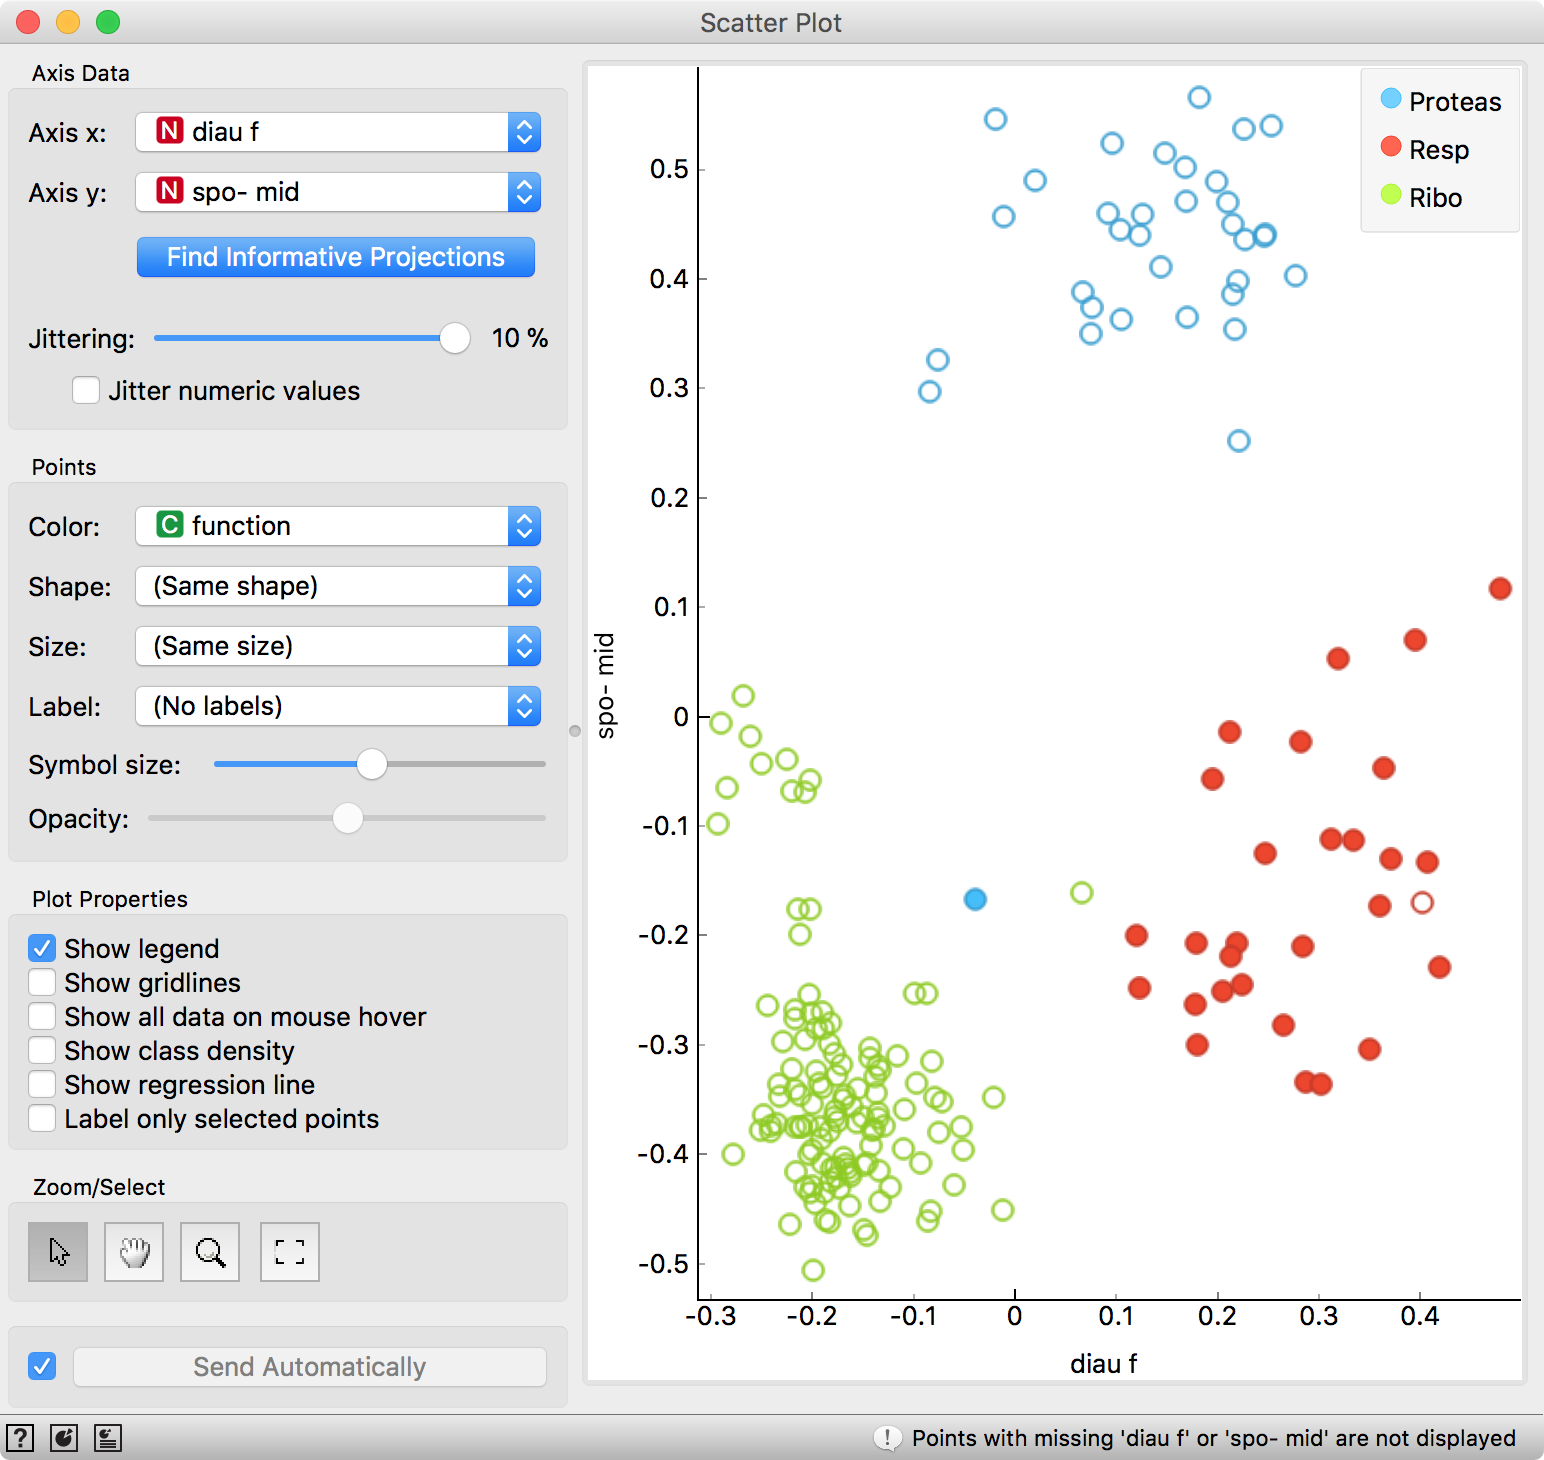
\includegraphics[width=0.95\linewidth]{scatterplot.png}
    \caption{$\;$}
\end{figure}